%% Daniel Ellison 2019
%% LaTeX

\documentclass{hitec}

\usepackage{courier}
\usepackage{textcomp}
\usepackage{tikz}

\title{Mini Projects: Lecture 5}
\author{Matthew Ellison}
\company{MIT/SPISE}

\begin{document}

\maketitle


\section{Estimating $\pi$}
Imagine a circle inside of a square as shown, with the circle centered at (0,0) of radius 1. If you were to throw darts randomly in the square region, the chance of a dart hitting inside the circle would be the ratio of the area of the circle to the entire region---$\frac{\pi}{4}$.
Write a simulation to choose many random points in the square region and compute the fraction which lie in the circle. This fraction is expected to be $\frac{\pi}{4}$, so multiply it by 4 at the end and you'll have made an estimate of pi!


\begin{center}
\tikzset{every picture/.style={line width=0.75pt}} %set default line width to 0.75pt        

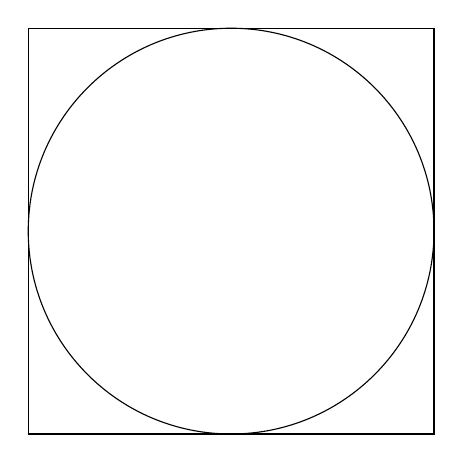
\begin{tikzpicture}[x=0.75pt,y=0.75pt,yscale=-1,xscale=1]
%uncomment if require: \path (0,300); %set diagram left start at 0, and has height of 300

%Shape: Circle [id:dp883733710411359] 
\draw   (236,140.75) .. controls (236,86.76) and (279.76,43) .. (333.75,43) .. controls (387.74,43) and (431.5,86.76) .. (431.5,140.75) .. controls (431.5,194.74) and (387.74,238.5) .. (333.75,238.5) .. controls (279.76,238.5) and (236,194.74) .. (236,140.75) -- cycle ;
%Shape: Square [id:dp7628170763224006] 
\draw   (236,43) -- (431.5,43) -- (431.5,238.5) -- (236,238.5) -- cycle ;

\end{tikzpicture}
\end{center}

\section{A Hard Probability Question (If You Don't Have A Computer)}
Begin with a count of 0. Choose a random decimal between 0 and 1 and add it to the count. Keep doing this until the count is greater than 1 for the first time. What is the expected value of the count when this happens (expected value means the average value when the experiment is performed many times)? Once you've obtained a good estimate, see if you can use it to guess the exact solution (which is in terms of a mathematical constant $e$, whose value is 2.71828...).

\noindent \emph{\textbf{Hint:} \texttt{random.random()} will generate a random number between 0 and 1.}


\section{Shuffling a Deck of Cards}
Imagine randomly shuffling a deck of playing cards. What are the chances that no cards are in their original position after the shuffle? Is your answer close to an expression involving the mathematical constant $e=2.71828\ldots$?

\noindent \emph{\textbf{Hint 1:} Since the suits and values are not important for the problem, it's easiest to represent a deck of cards as a simple list---such as \texttt{[0, 1, ..., 51]}}\\
\noindent \emph{\textbf{Hint 2:} The \texttt{random.shuffle()} function will make your life easier, if you choose to use it. Read the documentation online.}

\section{Meteorites}
Two meteorites fall randomly (and independently) into a 2 mile by 1 mile rectangular field. What are the chances the meteors land less than 1 mile apart? What about less than a 1/2 mile apart?

\section{Random Walk on Wall Street}
You own a stock valued at \$50. Each day, suppose there's a 40\% chance the valuation will go up by \$1 and a 60\% chance the valuation will go down by \$1. What's the chance that the stock will reaches a \$100 valuation before it drops to \$0 and is worthless?
Use \texttt{matplotlib} to make a chart of the value of the stock over time for a single run, until it falls to \$0 or reaches \$100. Give the plot a title and axis labels so it looks nice.

\end{document}